% results_ts.tex — Elicit vs. teach inside one model family (TinyStories-1B),
% organised by METRIC. Each metric has the same three blocks: "In one sentence"
% (what the metric asks, in plain words), "How it is measured" (the procedure,
% self-contained), "Elicit vs. teach" (the numbers, with a table or figure and a
% one-line reading). Figures are the PNGs generated by make_assets.py in this
% folder (paths relative to paper/). Every number has a dated entry in
% ../notes/decisions.md.
\documentclass[11pt]{article}
\usepackage{amsmath,amssymb}
\usepackage{graphicx}
\usepackage{booktabs}
\usepackage{adjustbox}
\usepackage[margin=1in]{geometry}
\usepackage{enumitem}
\usepackage{hyperref}
\newcommand{\what}[1]{\par\noindent\textbf{In one sentence.} #1}
\newcommand{\how}[1]{\par\noindent\textbf{How it is measured.} #1}
\newcommand{\numbers}[1]{\par\noindent\textbf{Elicit vs.\ teach.} #1\par\medskip}
\newcommand{\metricsec}[2]{\item \textbf{#1} --- \emph{#2}}

\title{Elicit vs.\ Teach, Mechanistically:\\ Eleven Metrics on the TinyStories-1B Twins}
\author{MARS V --- Mechanistic Understanding of Elicitation vs.\ Teaching}
\date{Working results document, September 2026}

\begin{document}
\maketitle

\section*{Setup}

\noindent\textbf{The experiment.} Two identical copies (``twins'') of a 1B-parameter language model
pretrained only on children's stories --- no arithmetic anywhere in the corpus --- are fine-tuned
on the same target task: natural-language addition and subtraction of 1--4-digit numbers,
\texttt{What is the difference between 8 and 5784?}$\;\to\;$\texttt{-5776}. The training protocol
is identical for both. The \emph{only} difference is the checkpoint the fine-tune starts from:

\begin{itemize}[nosep]
  \item \textbf{Teach twin}: the blank base model. The capability is absent.
  \item \textbf{Elicit twin} (``TS1B-latent''): the blank base plus two installations, neither of
    which shows the target task: (i) arithmetic in symbols only (\texttt{23 + 45 = 68}, 1M
    examples, full fine-tuning) and (ii) a word$\leftrightarrow$symbol binding dose that only
    \emph{rewrites} questions (\texttt{What is the sum of 621 and 5068?} $\leftrightarrow$
    \texttt{621 + 5068}) and never shows an answer. This twin can compute in symbols and knows
    what the words mean, but on the target task it scores $0.000$: asked a question, it rewrites
    it instead of answering. The capability is latent.
\end{itemize}

\noindent Every construction step has a control (Table~\ref{tab:premise}); the two twins are
behaviourally identical on the target task before fine-tuning.

\begin{table}[h]\centering\small
\begin{adjustbox}{max width=\textwidth}
\begin{tabular}{lcc}
\toprule
Construction step / check & value & control \\
\midrule
symbol install: exact match on \texttt{23 + 45 = } & 0.67--0.73 & blank twin: 0.00 \\
corpus census: ``sum'' in 439M words of stories & 21$\times$ & ``equals'' 17, ``minus'' 57 \\
binding dose: question $\to$ symbols rewrite exact & 0.484 & blank + same dose: 0.000 \\
sum-only dose on \emph{difference} questions & writes ``+'' & binding is per word \\
\textbf{exact match on the target task, before fine-tuning} & \textbf{0.000} & $=$ blank twin \\
\bottomrule
\end{tabular}
\end{adjustbox}
\caption{The elicit twin before fine-tuning: can compute in symbols, understands the words, still
answers nothing. Everything below is about what differs inside the two twins and what that
difference does.}
\label{tab:premise}
\end{table}

\noindent\textbf{Endpoints.} Seven fine-tuned models enter the results (Table~\ref{tab:endpoints}).
With the paper's adapter protocol (LoRA), the teach twin stops by the protocol's own
convergence rule far below the elicit twin --- $0.093$ with 1M examples and $0.139$ with four
times as many unique examples --- which is where the paper's own Figure~2 puts this model
(1--2 nats per token at 1M; ``stalls at lower accuracy''). Teaching this base needs full
fine-tuning. Two fully fine-tuned teach endpoints are carried through every metric: the
\emph{format-installed} twin (the paper's ``pre-teach format'' control: the blank base first
fine-tuned on a random-label dose in the target's own format, so it already emits a number after
every question; exact match $0.000$) fine-tuned to convergence, which reaches $0.424$; and the
blank twin fine-tuned to convergence, which reaches $0.819$. The elicit twin was fully
fine-tuned with the identical recipe ($0.986$). The format-installed pair is the design-matched
comparison --- both parents are the blank base plus a full-FT dose, both already output numbers,
only one has the algorithm --- and the blank-base pair is the better-performing one; the two
taught endpoints agree on every metric below. LoRA endpoints are kept as robustness rows; two
metrics need adapter snapshots (formation time, weight travel) and exist only for the LoRA runs.

\begin{table}[h]\centering\small
\begin{adjustbox}{max width=\textwidth}
\begin{tabular}{llllccc}
\toprule
endpoint & parent & method & data & steps (passes) & stop & exact match \\
\midrule
elicit LoRA & TS1B-latent & LoRA $r{=}512$ & 1M & 11{,}500 (1.5) & converged & \textbf{0.981} \\
teach LoRA 1M & blank & LoRA $r{=}512$ & 1M & 25{,}000 (3.2) & converged & 0.093 \\
teach LoRA 4M & blank & LoRA $r{=}512$ & 4M & 39{,}500 (1.3) & converged & 0.139 \\
teach FT & blank & full FT & 4M & 62{,}500 (2.0) & ceiling & 0.771 \\
teach FT, converged & blank & full FT & 4M & 72{,}000 (2.3) & converged & \textbf{0.819} \\
\textbf{teach FT, format-installed} & format-installed & full FT & 4M & 58{,}500 (1.9) & converged & \textbf{0.424} \\
\textbf{elicit FT} & TS1B-latent & full FT & 4M & 21{,}500 (0.7) & converged & \textbf{0.986} \\
\bottomrule
\end{tabular}
\end{adjustbox}
\caption{Fine-tuned endpoints. LoRA learning rate $3.53{\times}10^{-4}$, full FT $2{\times}10^{-5}$;
batch 128; seed 316; training stops when validation loss stops improving (eps/k rule). Exact
match $=$ 0-shot accuracy on 1,024 held-out problems. The 4M file is the 1M file plus 3M new
unique problems, disjoint from every evaluation set. ``Converged'' teach FT continues the
2-pass run from its checkpoint until the rule fires (optimizer state restarted).}
\label{tab:endpoints}
\end{table}

\noindent\textbf{Two terms used throughout.} \emph{Answer position}: the last prompt token, where
the model predicts the first token of the answer; every activation measurement is taken there
unless stated. \emph{Residual stream}: the model's running internal state at a token position, a
2048-dimensional vector that every layer reads and adds to. Everything else is defined where it
is used.

\noindent\textbf{How to read this document.} Eleven metrics, each with the same three blocks:
\textbf{In one sentence} (what the metric asks), \textbf{How it is measured} (the procedure,
complete enough to reproduce), \textbf{Elicit vs.\ teach} (the numbers). The metrics are grouped
by what they look at: the \emph{cost} of learning (M1), the \emph{machinery} that results
(M2--M4), the \emph{dynamics} of building it (M5--M8), and the \emph{latent state} before any
target training (M9--M11). Table~\ref{tab:ftpair} at the end puts every metric for the full-FT
endpoints on one page.

% =====================================================================
\section*{A. Cost of learning}
\begin{enumerate}[label=\textbf{M\arabic*}, leftmargin=*, itemsep=1.2em]

\metricsec{Learning cost}{cheaper with every example vs.\ the hump}
\what{How many extra nats it costs the model to learn each new example, and whether that cost
only falls (connecting something that exists) or first rises (building something new).}
\how{Prequential excess description length (EDL), the paper's learning-cost measure. Train on a
stream of $n$ examples; before each example is trained on, record the extra nats the model needs
to predict its answer tokens beyond a converged reference; sum over the stream and divide by the
number of answer tokens (EDL per token). Repeat on a sweep $n=100\ldots4{\times}10^6$ with the
identical LoRA protocol (19 rungs per arm, all converged), plus 0-shot exact match on 1,024
held-out problems at each rung. A falling curve means each example costs less than the last; a
down--up--down curve (``the hump'') means mid-run examples are the most informative because
structure is being built. Three arms: the elicit twin, the blank teach twin, and the
format-installed teach twin. The full-FT endpoints have no sweep; their cost is reported as steps
to convergence and held-out test loss.}
\numbers{Figure~\ref{fig:flip}, Table~\ref{tab:sweep}. \textbf{Elicit}: strictly monotone
decreasing, $4.53\to0.092$ nats; exact match $0.54$ already at $n{=}3{,}162$, $0.98$ at 1M.
\textbf{Teach} (blank): down--up--down, minimum $0.78$ at $14.7$K, peak $2.02$ at $215$K, $1.40$
at 1M; exact match $0.093$ at 1M and $0.139$ at 4M. \textbf{Teach} (format-installed): the same
hump with the format cost prepaid, minimum $0.64$ at 10K, peak $1.33$ at 100K, $0.88$ at 1M,
exact match $0.079$. The dataset size at which exact match crosses 0.5 differs by more than
$300\times$. Full FT: elicit converges in 21,500 steps (0.7 of a pass, test loss $0.015$, exact
match $0.986$); blank teach runs to the two-pass ceiling ($0.771$) and converges 9,500 steps
later at $0.819$ (test loss $0.154$); format-installed teach converges after 58,500 steps at
$0.424$ (test loss $0.639$). \emph{Reading:} eliciting spends every example connecting a
capability that already exists; teaching has to build it, so the cost rises mid-run and the
model converges lower after three times the steps --- and the hump survives removing the format,
so it is the algorithm being built.}
\begin{figure}[h]\centering
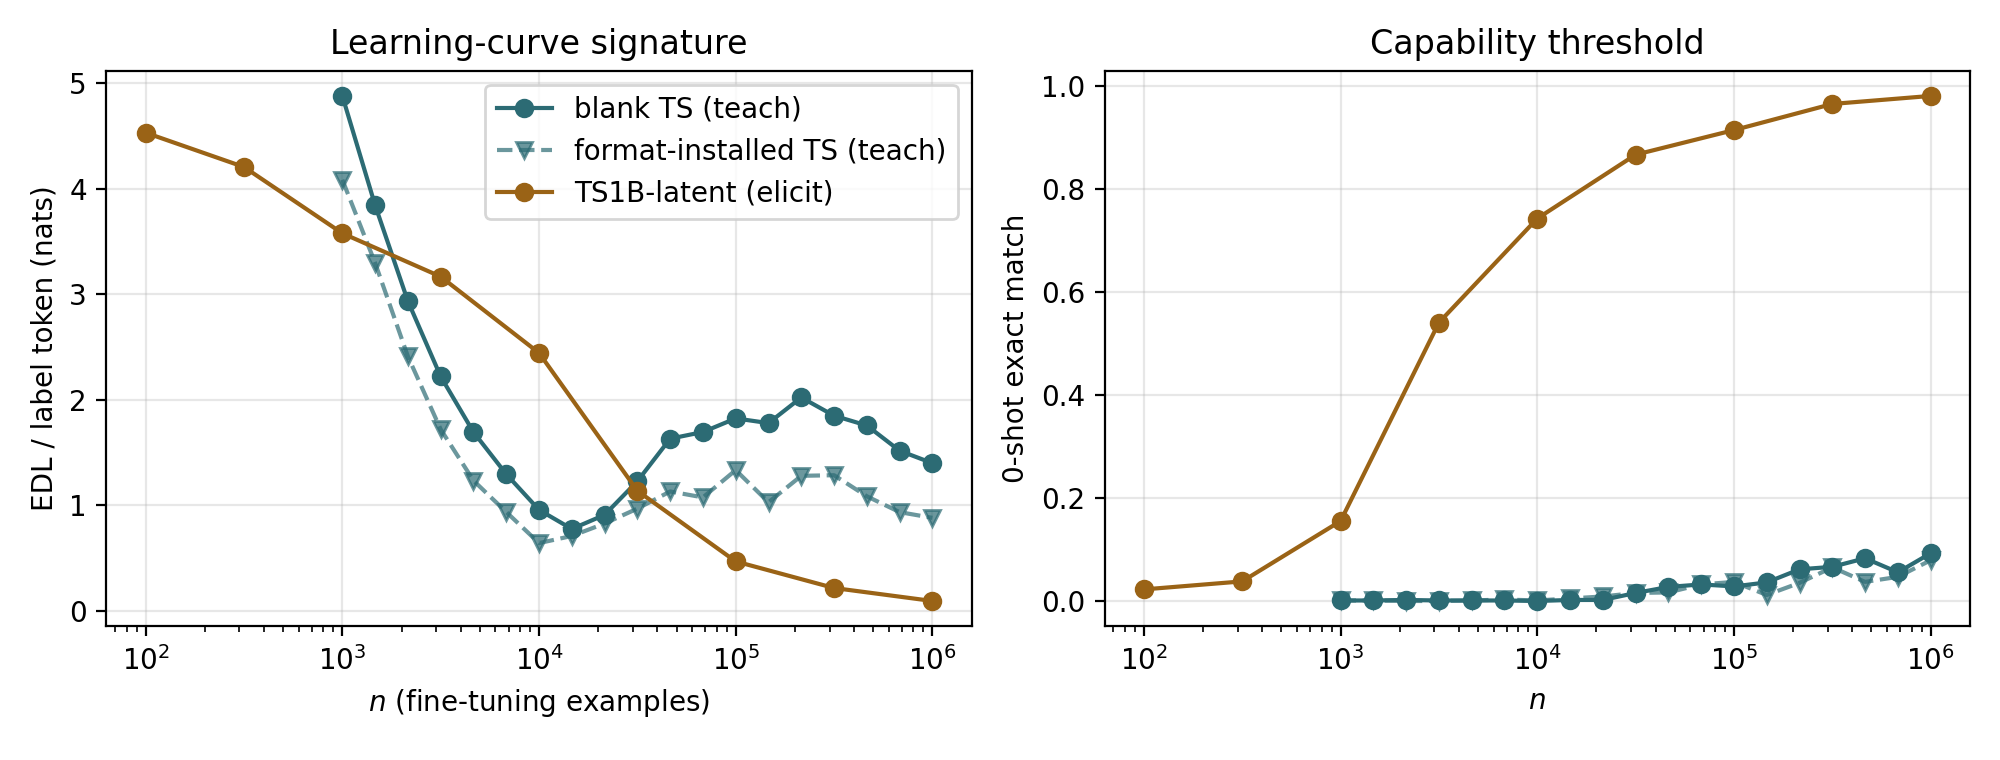
\includegraphics[width=\textwidth]{02_learning_curves/fig_signature_flip.png}
\caption{EDL/token (left) and 0-shot exact match (right) vs $n$; teal = teach twin from the blank base, dashed teal = teach twin from the format-installed base, gold = elicit twin.}
\label{fig:flip}
\end{figure}
\begin{table}[h]\centering\small
\begin{adjustbox}{max width=\textwidth}
\begin{tabular}{rcccccc}
\toprule
$n$ & \multicolumn{2}{c}{elicit (TS1B-latent)} & \multicolumn{2}{c}{teach (blank)} & \multicolumn{2}{c}{teach (format-installed)} \\
 & EDL/tok & EM & EDL/tok & EM & EDL/tok & EM \\
\midrule
100 & 4.533 & 0.023 & 6.511 & 0.007 & -- & -- \\
316 & 4.208 & 0.038 & 6.387 & 0.033 & -- & -- \\
1{,}000 & 3.579 & 0.155 & 4.882 & 0.001 & 4.087 & 0.001 \\
3{,}162 & 3.168 & \textbf{0.541} & 2.221 & 0.001 & 1.720 & 0.000 \\
10{,}000 & 2.444 & 0.743 & 0.956 & 0.000 & \emph{0.641} (min) & 0.001 \\
14{,}678 & -- & -- & \emph{0.775} (min) & 0.002 & 0.708 & 0.005 \\
31{,}623 & 1.137 & 0.867 & 1.228 & 0.016 & 0.968 & 0.016 \\
100{,}000 & 0.467 & 0.915 & 1.824 & 0.028 & \emph{1.333} (peak) & 0.037 \\
215{,}443 & -- & -- & \emph{2.022} (peak) & 0.062 & 1.279 & 0.035 \\
316{,}228 & 0.215 & 0.966 & 1.849 & 0.066 & 1.285 & 0.065 \\
1{,}000{,}000 & \textbf{0.092} & \textbf{0.981} & 1.399 & 0.093 & 0.880 & 0.079 \\
4{,}000{,}000 & -- & -- & 0.930 & 0.139 & -- & -- \\
\bottomrule
\end{tabular}
\end{adjustbox}
\caption{Per-rung values, LoRA protocol (EDL in nats per answer token; EM $=$ exact match; 19
rungs per teach arm, all converged; rungs shared with the elicit sweep shown plus each arm's
minimum and peak).}
\label{tab:sweep}
\end{table}

% =====================================================================
\end{enumerate}
\section*{B. The machinery that results}
\begin{enumerate}[label=\textbf{M\arabic*}, leftmargin=*, itemsep=1.2em, resume]

\metricsec{Circuit overlap}{the same circuit vs.\ a new circuit}
\what{Whether two models solve the task with the same set of components, read against how
repeatable a circuit is at all.}
\how{\emph{Building a circuit.} The model is split into 528 nodes: 512 attention heads (32 per
layer $\times$ 16 layers; heads move information between token positions) and 16 MLP blocks (one
per layer; they transform it in place). For each node, attribution patching scores how much the
answer's logit would change if that node's activation at the answer position were replaced by its
value on a different problem: gradient of the answer logit-difference with respect to the node's
activation, times the activation difference between the clean and the corrupted problem, averaged
over 128--256 problem pairs. The 32 highest-scoring nodes are the circuit. A model that cannot do
the task gives a noise map, which the tool flags (its answer logit-difference is $\approx0$).
\emph{Comparing circuits.} Jaccard@32 $=$ shared nodes $\div$ union of the two 32-node sets. Two
random circuits overlap at $0.031$. The \emph{ceiling} is the overlap of two circuits of the
\emph{same} model computed from two disjoint halves of the data --- how repeatable a circuit is
($0.42$--$0.68$ here); an overlap at the ceiling means ``the same circuit''. Spearman $=$ rank
correlation of the node scores over the union. Also the layer histogram of each circuit's top-16
nodes, and for the LoRA-1M pair the change at the level of connections between nodes (edge-level
$\Delta S = 1-\text{Jaccard}$ over the 256 strongest node$\to$block edges).}
\numbers{Table~\ref{tab:overlap}, Figure~\ref{fig:layers}. \textbf{Parent $\to$ child.} The
elicit parent's symbol circuit $\leftrightarrow$ its child's natural-language circuit: $0.455$--$0.524$
(about 70\% of the ceiling), and the top four nodes are the same four in the same order
(\texttt{mlp:15,14,13,12}); the shared backbone is complete at $n{=}3$K (child@3K
$\leftrightarrow$ child@1M: $0.391$). The blank parent has no measurable circuit (logit-diff
$-0.33$ even with 16 examples in the prompt), so the taught child has nothing to reuse.
\textbf{Child $\leftrightarrow$ child.} The two elicited children --- one LoRA, one full FT ---
overlap at $0.641$, at the ceiling: one circuit whichever way it is trained. Every taught child
sits apart from them: $0.306$ for the format-installed full-FT pair (Spearman $0.03$), $0.333$
for the blank-base full-FT pair, $0.391$ for the LoRA-4M pair, $0.231$ for the LoRA-1M pair ---
about 60\% of the ceiling, score correlations between $-0.11$ and $0.28$. Taught children agree
with each other at $0.36$--$0.60$. What all circuits share is the late-layer MLP engine
(\texttt{mlp:15,14,13,7}); what differs is the rest: taught circuits add \texttt{mlp:0,10,11}
(the format-installed one also \texttt{mlp:1,3,4,5,6}) and their own attention heads (eight
layer-0 heads over the raw digits under LoRA; heads in layers 4--7 and 15 under full FT),
elicited circuits use \texttt{mlp:8,9} and three layer-7 heads. LoRA-1M pair:
$\Delta S_{\text{node}}=0.769$, $\Delta S_{\text{edge}}=0.739$, both far above the noise floors
(0.32 / 0.61). \emph{Reading:} elicitation re-weights the circuit the parent already had;
teaching builds a related but different one --- the same late-layer MLPs, its own way of
fetching and routing the operands.}
\begin{table}[h]\centering\small
\begin{adjustbox}{max width=\textwidth}
\begin{tabular}{lccc}
\toprule
Comparison & Jaccard@32 & chance & ceiling(s) \\
\midrule
parent's symbol circuit $\leftrightarrow$ elicited child (two eval surfaces) & 0.455--0.488 / 0.524 & 0.031 & 0.684 \\
elicited child @3K $\leftrightarrow$ @1M & 0.391 & 0.031 & 0.684 \\
elicited child, full FT $\leftrightarrow$ elicited child, LoRA & \textbf{0.641} (Spearman 0.54) & 0.031 & 0.561 / 0.684 \\
blank parent $\leftrightarrow$ taught child & undefined (parent map is noise) & -- & -- \\
elicited FT $\leftrightarrow$ taught FT, format-installed & 0.306 (Spearman 0.03) & 0.031 & 0.561 / 0.524 \\
elicited FT $\leftrightarrow$ taught FT, blank, 2 passes / converged & 0.333 (Spearman 0.16) / 0.333 (0.28) & 0.031 & 0.561 / 0.422 \\
taught FT, converged $\leftrightarrow$ taught FT before continuation & 0.600 (Spearman 0.57) & 0.031 & 0.422 / 0.422 \\
taught FT, format-installed $\leftrightarrow$ taught FT, blank, converged & 0.362 (Spearman 0.18) & 0.031 & 0.524 / 0.422 \\
elicited $\leftrightarrow$ taught, LoRA pair (4M) & 0.391 (Spearman 0.28) & 0.031 & 0.684 / 0.524 \\
elicited $\leftrightarrow$ taught, LoRA pair (1M) & 0.231 (Spearman $-0.11$) & 0.031 & 0.684 / 0.561 \\
taught, full FT $\leftrightarrow$ taught, LoRA 4M & 0.391 (Spearman 0.11) & 0.031 & 0.422 / 0.524 \\
\bottomrule
\end{tabular}
\end{adjustbox}
\caption{Circuit overlaps. All maps pass the performing-regime check.}
\label{tab:overlap}
\end{table}
\begin{figure}[h]\centering
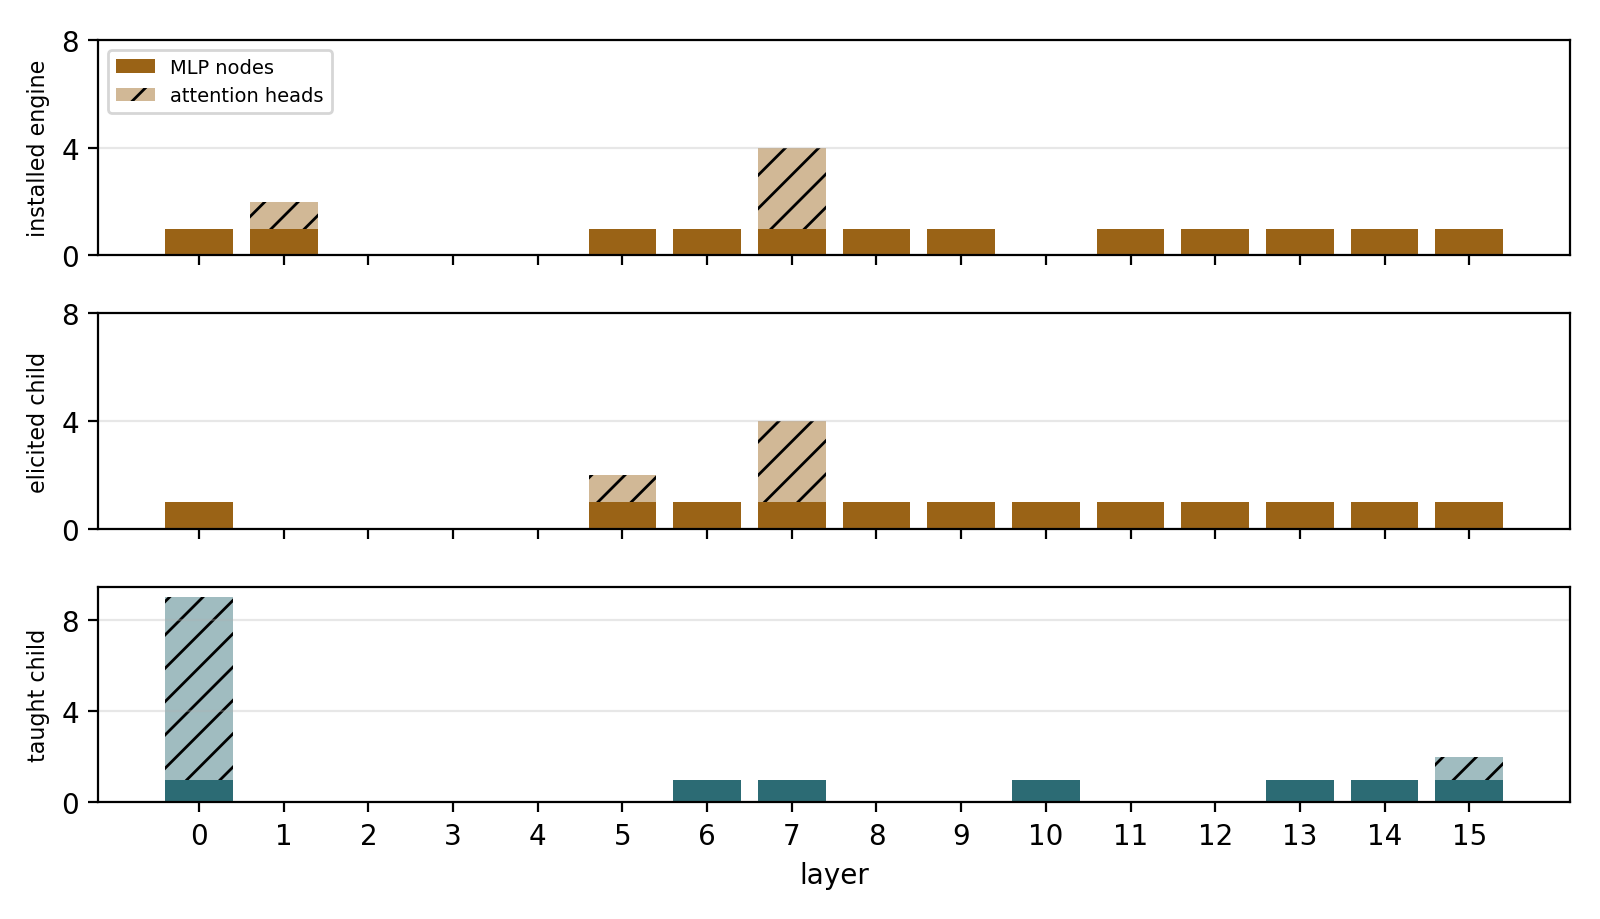
\includegraphics[width=0.9\textwidth]{03_circuits/fig_layer_profile_ts.png}
\caption{Top-16 node layer histograms (solid = MLP, hatched = attention) for the parent's symbol circuit, the LoRA-elicited child and the LoRA-1M taught child.}
\label{fig:layers}
\end{figure}

\metricsec{Circuit faithfulness}{does the circuit carry the computation?}
\what{Whether the 32 nodes called ``the circuit'' really produce the answer --- the check that
licenses every overlap in M2 as a comparison between two real mechanisms.}
\how{True activation patching, in two directions. \emph{Sufficiency}: run a corrupted problem,
copy the clean problem's activations into only the top-$k$ nodes, and measure what fraction of
the clean-vs-corrupt answer logit-difference is recovered. \emph{Necessity}: run the clean
problem, corrupt only the top-$k$ nodes, and measure what fraction is destroyed. 128 problem
pairs, $k=8,16,32,64,128,528$; $1.0$ means the top-$k$ nodes alone account for the whole
behaviour.}
\numbers{Top-8 of 528 nodes recover / destroy the answer at: LoRA-elicited $0.997$ / $0.998$;
full-FT elicited $0.923$ / $0.943$; full-FT taught $0.950$ / $0.966$ (converged $0.950$ /
$0.965$; format-installed $0.983$ / $0.988$); LoRA-4M taught $0.976$ / $0.987$. Top-32
$\ge0.996$ everywhere. \emph{Reading:} the regimes do not differ here --- both build compact
circuits that are near-totally sufficient and necessary --- so the differences in M2, M4 and
M5 are differences between two load-bearing circuits, not between a circuit and noise.}

\metricsec{Head roles}{the same reader heads vs.\ rediscovered ones}
\what{Which attention heads carry each piece of the problem --- the first number, the second
number, the operation --- and whether a fine-tuned model keeps the parent's readers or has to
find its own.}
\how{Desiderata Component Masking (Prakash et al.\ 2024). For one piece of information at a
time, take a problem and a counterfactual problem that differs only in that piece, and learn
(by gradient descent on a mask over heads, with a sparsity penalty) the smallest set of
attention heads such that copying those heads' activations from the counterfactual run into the
clean run makes the model answer the counterfactual problem. That set is the heads carrying that
piece (its ``role''). The set is validated by its counterfactual-flip accuracy against the
ceiling obtained by copying every head; a set is ``compact'' only if it reaches that ceiling.
Role sets are compared across models by Jaccard (chance $\approx0.05$); 64--128 counterfactual
pairs, heads only.}
\numbers{Table~\ref{tab:dcm}. \textbf{Elicit}: parent $\leftrightarrow$ LoRA-elicited child, flip
accuracy at the ceiling for every set, first operand $0.879$ (29 of 33 heads shared), second
operand $0.900$, operation $0.750$; the operand heads are almost all layer-0 attention (30 of 32).
The full-FT elicited child keeps the same heads ($0.811$ / $0.833$ vs the LoRA child, $0.694$ /
$0.857$ vs the parent). \textbf{Teach}: every performing taught model has compact operand sets at
its ceiling, overlapping the parent's engine at $0.76$--$0.88$ (first operand) / $0.66$--$0.68$
(second) and the elicited child's at $0.59$--$0.66$ / $0.69$--$0.76$; the full-FT taught set
contains 28 of the full-FT elicited child's 31 first-operand heads and adds nine more. The two
LoRA-taught children that never learned the task (exact match 0.09 / 0.14) have no compact set at
all: best flip accuracy $0.008$--$0.04$ against ceilings of $0.14$--$0.20$. \emph{Reading:}
operand reading is a layer-0 function of the substrate, so every model that solves the task uses
largely the same reader heads; elicitation keeps the parent's set nearly intact ($0.88$--$0.90$),
teaching rediscovers it and lands on a larger set ($0.6$--$0.88$) --- a graded difference.}
\begin{table}[h]\centering\small
\begin{adjustbox}{max width=\textwidth}
\begin{tabular}{lcccc}
\toprule
Comparison (first operand / second operand) & $|A|$ & $|B|$ & Jaccard & flip acc.\ / ceiling \\
\midrule
parent $\leftrightarrow$ elicited (LoRA), symbol surface & 30 / 27 & 32 / 30 & \textbf{0.879 / 0.900} & at ceiling \\
parent $\leftrightarrow$ elicited (LoRA), operation & 25 & 24 & \textbf{0.750} & at ceiling \\
elicited (full FT) $\leftrightarrow$ elicited (LoRA) & 31 / 25 & 36 / 30 & 0.811 / 0.833 & 0.98 / 0.98 \\
elicited (full FT) $\leftrightarrow$ parent & 31 / 25 & 30 / 27 & 0.694 / 0.857 & -- \\
taught (full FT) $\leftrightarrow$ elicited (LoRA) & 37 / 37 & 36 / 30 & 0.587 / 0.763 & 0.81 / 0.79 (0.81 / 0.80) \\
taught (full FT) $\leftrightarrow$ elicited (full FT) & 37 / 37 & 31 / 25 & 0.700 / 0.632 & -- \\
taught (full FT) $\leftrightarrow$ parent & 37 / 37 & 30 / 27 & 0.763 / 0.684 & -- \\
taught (FT, format-installed) $\leftrightarrow$ parent & 32 / 41 & 30 / 27 & 0.879 / 0.659 & 0.59 / 0.54 (0.59 / 0.55) \\
taught (FT, format-installed) $\leftrightarrow$ elicited (LoRA) & 32 / 41 & 36 / 30 & 0.659 / 0.690 & -- \\
taught (FT, blank, converged) $\leftrightarrow$ parent & 37 / 36 & 30 / 27 & 0.763 / 0.658 & 0.85 / 0.81 (0.85 / 0.83) \\
taught (FT, blank, converged) $\leftrightarrow$ elicited (LoRA) & 37 / 36 & 36 / 30 & 0.587 / 0.737 & -- \\
taught (LoRA 4M) $\leftrightarrow$ elicited (LoRA) & 12 / 21 & 36 / 30 & 0.043 / 0.041 & 0.01 / 0.03 (0.20 / 0.14) \\
taught (LoRA 1M) $\leftrightarrow$ elicited (LoRA) & 9 / 21 & 36 / 30 & 0.125 / 0.085 & 0.02 / 0.04 (0.15) \\
\bottomrule
\end{tabular}
\end{adjustbox}
\caption{Head roles by Desiderata Component Masking. $|A|$, $|B|$ $=$ size of the two role sets;
flip accuracy is reported for set $A$.}
\label{tab:dcm}
\end{table}

% =====================================================================
\end{enumerate}
\section*{C. Dynamics: how the machinery comes into being}
\begin{enumerate}[label=\textbf{M\arabic*}, leftmargin=*, itemsep=1.2em, resume]

\metricsec{Circuit formation time}{present at step 1 vs.\ assembled mid-run}
\what{When during training the final circuit comes into existence.}
\how{Adapter snapshots were saved along the LoRA runs (128 per run, log-spaced). For each
snapshot, build the circuit exactly as in M2 and take its Jaccard@32 with the run's final
circuit; read against chance ($0.031$) and the split-half ceiling. The step at which the curve
leaves the noise floor is when the circuit starts to exist; the step at which it reaches the
ceiling is when it stops changing.}
\numbers{Figure~\ref{fig:form}. \textbf{Elicit}: $0.488$ at step 1 ($16\times$ chance), a brief
dip to $\sim0.42$ while the input interface is wired (step 154), then locked from about step 1.5K
of 11.5K ($0.561$; 82\% of the ceiling, 97\% of the Jaccard@64 ceiling by 8.4K). \textbf{Teach}
(LoRA 1M): at the noise floor ($0.22$--$0.28$) until about step 1.3K, then $0.27\to0.44$ over
steps 1.3K--5.4K --- the region where its EDL peaks (M1). Teach (LoRA 4M): about a third of
the endpoint set from step 1 ($0.33$--$0.46$ against a $0.52$ ceiling), the rest churning to the
end ($0.36$ at 8K and 37K; logit-diff $0.9\to13.6$). \emph{Reading:} the elicited circuit is
present before training starts and stops changing by one-eighth of the run; the taught circuit
does not exist until a thousand steps in and is built exactly while the learning cost is rising.}
\begin{figure}[h]\centering
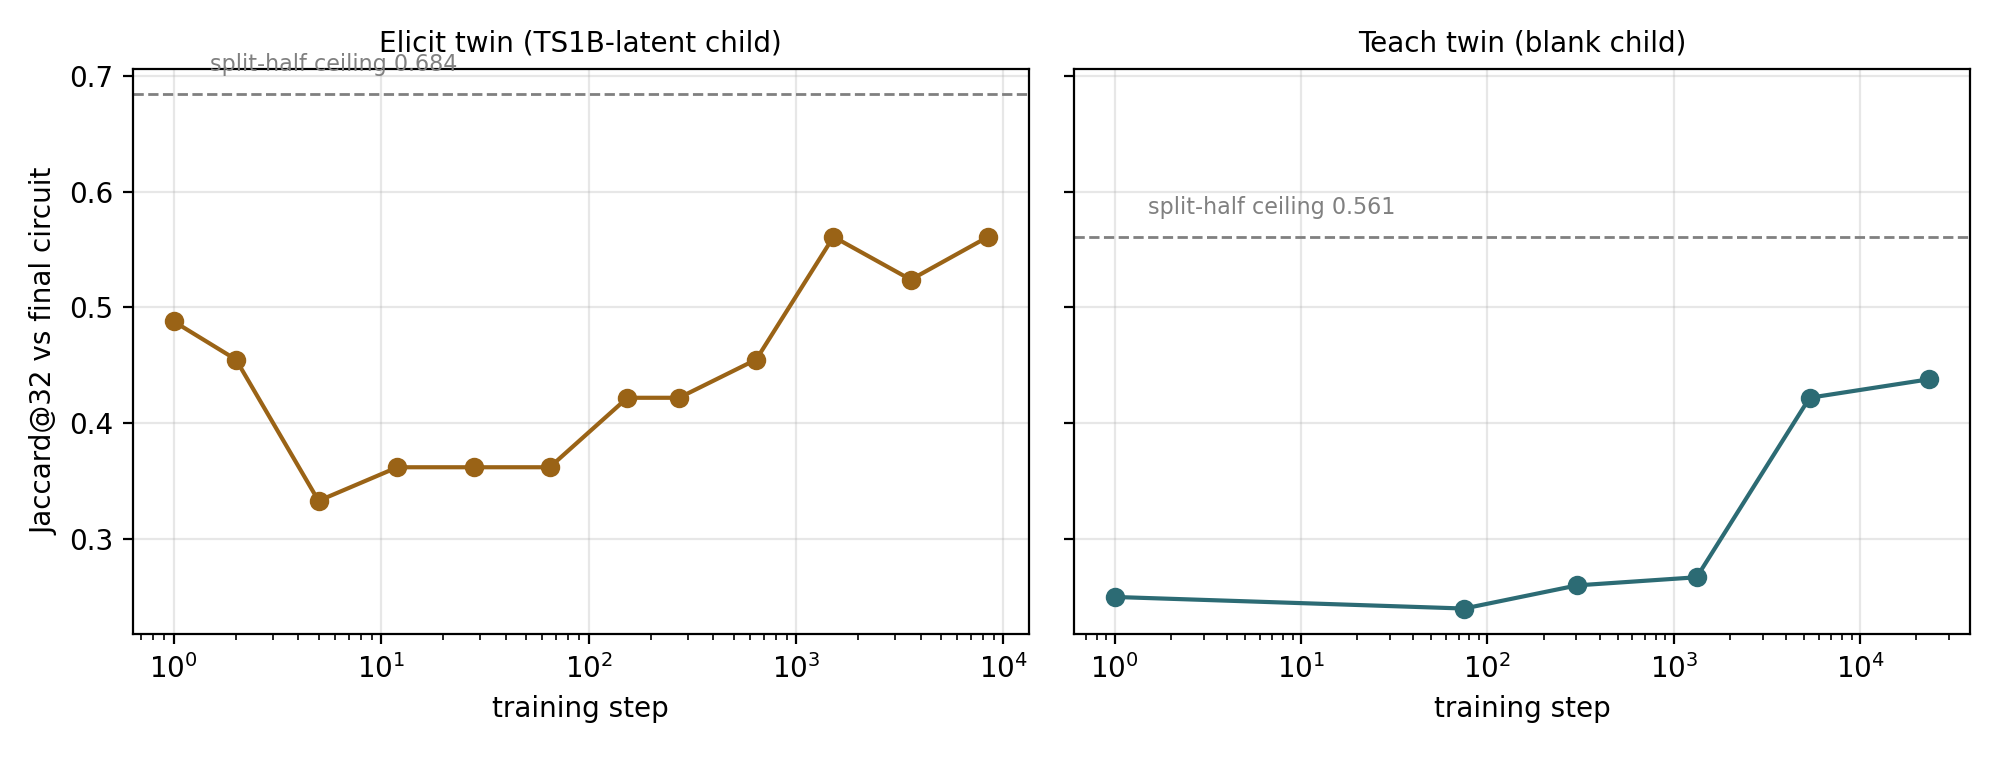
\includegraphics[width=\textwidth]{03_circuits/fig_formation_ts.png}
\caption{Circuit formation, elicit (left) vs teach (right); dashed = split-half ceiling.}
\label{fig:form}
\end{figure}

\metricsec{Gradient pressure}{a dying gradient vs.\ a growing one}
\what{How hard training is pushing on the weights, and whether that push fades (nothing left to
change) or grows (structure still being built).}
\how{The global gradient norm before clipping, logged at every update. Reported: its peak and
the step of the peak; its mean over the first 1\%, the middle, and the last 10\% of steps; the
ratio first-1\% $\div$ last-10\% (above 1 $=$ decays, below 1 $=$ grows); and the cumulative
gradient mass $\sum_t\|g_t\|$. For the LoRA runs also how that mass splits across attention
query/key weights (QK), attention value/output weights (VO) and MLP weights; the full-FT trainer
logs the global norm only. Norms are comparable within a method, not across methods (different
parameter sets).}
\numbers{Table~\ref{tab:grad}, Figure~\ref{fig:grad}. \textbf{LoRA.} Both arms start at the same
scale (first-1\% mean $0.18$ vs $0.17$). Elicit decays $3.3\times$ to a floor of $0.056$ (peak
$0.44$ at step 96). Teach grows $40$--$50\times$: last-10\% mean $6.8$ at 1M and $7.8$ at 4M,
peaks of $17.4$ and $22.0$ near the end. Cumulative mass $783$ vs $116{,}877$ (1M) and
$220{,}685$ (4M): $150$--$280\times$. Across the sweep the arms are indistinguishable up to
$n{=}10$K and diverge from $31.6$K. Teach's mass moves out of the MLPs (share $0.47\to0.01$) into
attention (VO share $0.87$ at 1M, $0.93$ at 4M). \textbf{Full FT.} Elicit peaks at step 1
($34.0$) and decays $3.4\times$ to a floor of $1.4$. Teach from the blank base starts lower
($2.3$), peaks at step 3,844 ($32.0$), holds $5.3$ mid-run and ends at $3.4$ ($1.5\times$ its
start); mass $353{,}277$ vs $44{,}021$ ($8\times$; $2.8\times$ per step over $2.9\times$ the
steps); the continuation adds 9,500 steps at a flat norm ($30{,}954$ more). Teach from the
format-installed parent: $2.69$ at the start, peak $70.9$ at step 50,860 (the largest single
update anywhere), $3.77$ at the end ($1.4\times$); mass $378{,}170$ ($8.6\times$ elicit).
\emph{Reading:} elicitation converges and its gradient dies, by the same $3.3$--$3.4\times$ under
either method; teaching generates gradient pressure that grows with the structure being built
--- $40$--$50\times$ under LoRA, $1.4$--$1.5\times$ under full FT --- and under LoRA aims it at the
attention weights where the operand-fetching heads of M4 are being written.}
\begin{table}[h]\centering\small
\begin{adjustbox}{max width=\textwidth}
\begin{tabular}{lcccccc}
\toprule
 & elicit LoRA 1M & teach LoRA 1M & teach LoRA 4M & elicit FT & teach FT, blank (+ cont.) & teach FT, format-inst. \\
\midrule
steps & 11{,}500 & 25{,}000 & 39{,}500 & 21{,}500 & 62{,}500 (+ 9{,}500) & 58{,}500 \\
peak gradient norm (step) & 0.441 (96) & 17.4 (23{,}657) & 22.0 (36{,}931) & 34.0 (1) & 32.0 (3{,}844) & 70.9 (50{,}860) \\
mean norm: first 1\% / middle / last 10\% & 0.183 / 0.060 / 0.056 & 0.169 / 5.21 / 6.80 & 0.160 / 6.61 / 7.78 & 4.80 / 1.85 / 1.39 & 2.30 / 5.31 / 3.43 & 2.69 / 4.86 / 3.77 \\
first 1\% $\div$ last 10\% & $\times$3.3 (decays) & $\times$0.02 (grows $\sim$40$\times$) & $\times$0.02 (grows $\sim$50$\times$) & $\times$3.4 (decays) & $\times$0.7 (grows 1.5$\times$) & $\times$0.7 (grows 1.4$\times$) \\
cumulative gradient mass $\sum_t\|g_t\|$ & 783 & 116{,}877 & 220{,}685 & 44{,}021 & 353{,}277 (+ 30{,}954) & 378{,}170 \\
gradient mass per step & 0.068 & 4.68 & 5.59 & 2.05 & 5.65 (3.26) & 6.46 \\
mass share QK / VO / MLP & .18 / .55 / .27 & .12 / .87 / .01 & .05 / .93 / .01 & -- & -- & -- \\
\bottomrule
\end{tabular}
\end{adjustbox}
\caption{Raw gradient strength (pre-clip global norm at every update). LoRA and full-FT norms are
on different parameter sets and are compared within a method only.}
\label{tab:grad}
\end{table}
\begin{figure}[h]\centering
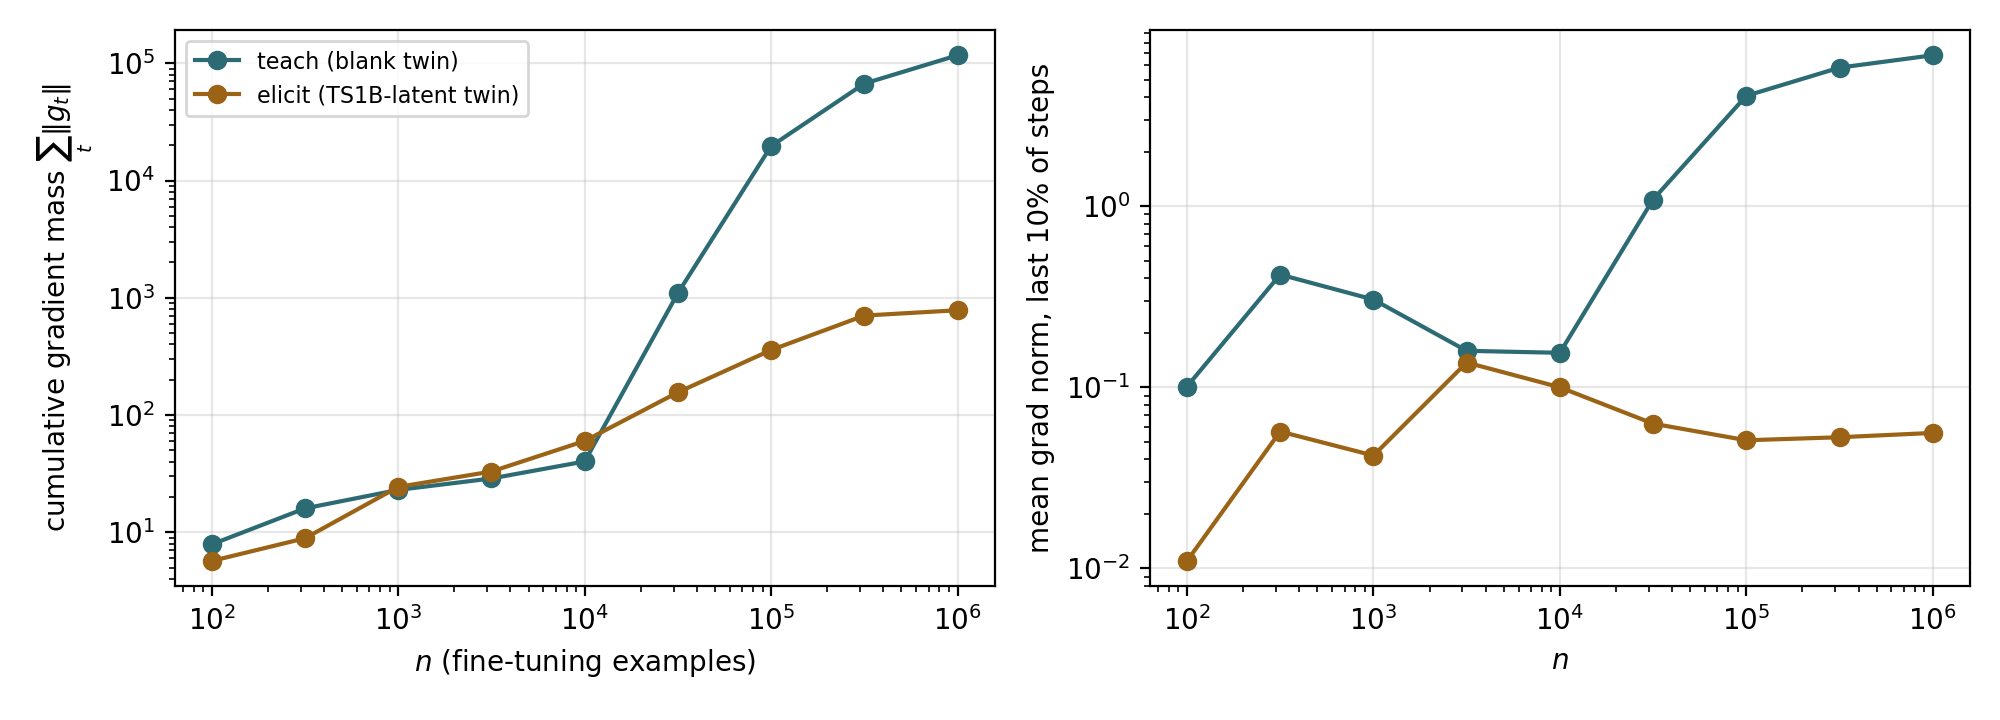
\includegraphics[width=\textwidth]{05_weights/fig_grad_strength.png}
\caption{Cumulative gradient mass (left) and late-run gradient norm (right) vs $n$; teal = teach, gold = elicit.}
\label{fig:grad}
\end{figure}

\metricsec{Weight write}{a small update vs.\ a large one}
\what{How much fine-tuning changes the weights, how far they travel to get there, and how much
capability each unit of change buys.}
\how{Relative weight change $\|\Delta W\|/\|W\|$ between child and parent --- exact from the LoRA
factors ($\Delta W = BA$), or from the checkpoint difference for full fine-tuning --- over all
attention and MLP matrices, with the effective rank of $\Delta W$ (participation ratio of its
spectrum; 2048 $=$ full rank). Along the LoRA runs, from the adapter snapshots: total travel
$\|\Delta W_t\|_F$ vs step, its peak and final speed per step, and capability per unit travel
$=$ final exact match $\div$ total travel.}
\numbers{Table~\ref{tab:weights}. \textbf{LoRA}: relative write $0.212$ (teach 1M) and $0.264$
(teach 4M) vs $0.095$ (elicit), $2.2$--$2.8\times$; total travel $457$ vs $120$ ($3.8\times$)
over twice as many steps; capability per unit travel $2.0\times10^{-4}$ vs $8.1\times10^{-3}$
($\sim40\times$). \textbf{Full FT}, no adapters involved: $0.094$ (teach, blank, 2 passes),
$0.102$ (converged), $0.086$ (format-installed parent) vs $0.050$ (elicit), $1.7$--$2.0\times$,
with the same effective rank of the change ($480$--$580$ vs $554$). The travel \emph{profile}
is the same in both arms (a burst, then decay): the optimiser's normalisation compresses the
$150\times$ gradient gap of M6 into a $3.8\times$ step-size gap. \emph{Reading:} teaching
writes two to four times more into the weights than elicitation and gets forty times less
capability per unit written, under both methods --- eliciting connects what exists, teaching
writes what does not.}
\begin{table}[h]\centering\small
\begin{adjustbox}{max width=\textwidth}
\begin{tabular}{lcc}
\toprule
 & elicit (TS1B-latent) & teach (blank) \\
\midrule
relative write $\|\Delta W\|/\|W\|$, LoRA 1M & 0.095 & 0.212 \\
relative write, LoRA 4M & -- & 0.264 \\
relative write, full FT (4M): blank 2 passes / converged / format-installed & 0.050 & 0.094 / 0.102 / 0.086 \\
effective rank of $\Delta W$, full FT (of 2048) & 554 & 571 / 580 / 481 \\
steps to convergence (LoRA 1M) & 11{,}500 & 23{,}496 \\
peak / final writing speed per step (LoRA 1M) & 0.218 / 0.018 & 0.306 / 0.022 \\
total weight travel $\|\Delta W\|_F$ (LoRA 1M) & 120 & 457 \\
final exact match (LoRA 1M) & 0.981 & 0.093 \\
capability per unit travel (LoRA 1M) & $8.1\times10^{-3}$ & $2.0\times10^{-4}$ \\
\bottomrule
\end{tabular}
\end{adjustbox}
\caption{Weight-space write, elicit vs teach (travel curves in \texttt{05\_weights/fig\_weight\_travel}).}
\label{tab:weights}
\end{table}

\metricsec{State-shift direction}{a different vector per problem vs.\ one shared vector}
\what{Whether fine-tuning changes the model's internal state by something problem-specific (the
answer, routed to the output) or by the same push on every problem (moving the model into a new
mode).}
\how{Run the same 256 problems through parent and child (both in fp32) and take the difference
of their residual streams at the answer position, layer by layer. \emph{Size}: its norm relative
to the parent's state. \emph{Direction}: stack the 256 difference vectors and compute the
fraction of their energy in the single best direction (PC1; $1.0$ means every problem's
difference is the same vector). The reference for ``unrelated vectors'' is the PC1 of the
parent's own 256 states, given alongside. The same PC1 is recomputed after projecting out the
directions that encode the answer token and the parent's top-1 token, so that ``the same vector''
cannot simply be the answer. Also the cosine of each shift to the mean shift, and, as a functional
counterpart, KL(parent$\|$child) at the answer position vs on generic story text.}
\numbers{Figure~\ref{fig:resid}, Table~\ref{tab:resid}. \textbf{Elicit}: PC1 of the shift at
the read-out $0.063$ (LoRA) and $0.056$ (full FT), with the parent's own states at $0.23$ --- no
shared direction. \textbf{Teach}: $0.528$ (LoRA 4M), $0.521$ / $0.526$ (full FT from the blank
base, 2 passes / converged) and $0.567$ from the format-installed parent, still $0.52$--$0.56$
after the answer-token directions are removed. The format-installed parent already emits a
number after every question, so its child has no output format to learn --- and its shift
carries the largest shared component: the component is the algorithm's mode, not the format.
Cosine to the mean shift: elicit $0.26$ / $0.23$, teach $0.26$ / $0.74$ / $0.80$. Size and depth
follow the fine-tuning method, not the regime (LoRA-taught final-layer write $14$--$29\times$
the parent's norm, full-FT $1.2$--$1.4\times$, elicit $1.7$--$1.9\times$). \emph{Reading:}
elicitation changes the state by a problem-specific vector because the parent already sits in a
problem-specific state; teaching's change is dominated by one shared component because the blank
parent's state at the answer position carries no problem information and the model has to be
moved into answering mode before any content can be added.}
\begin{figure}[h]\centering
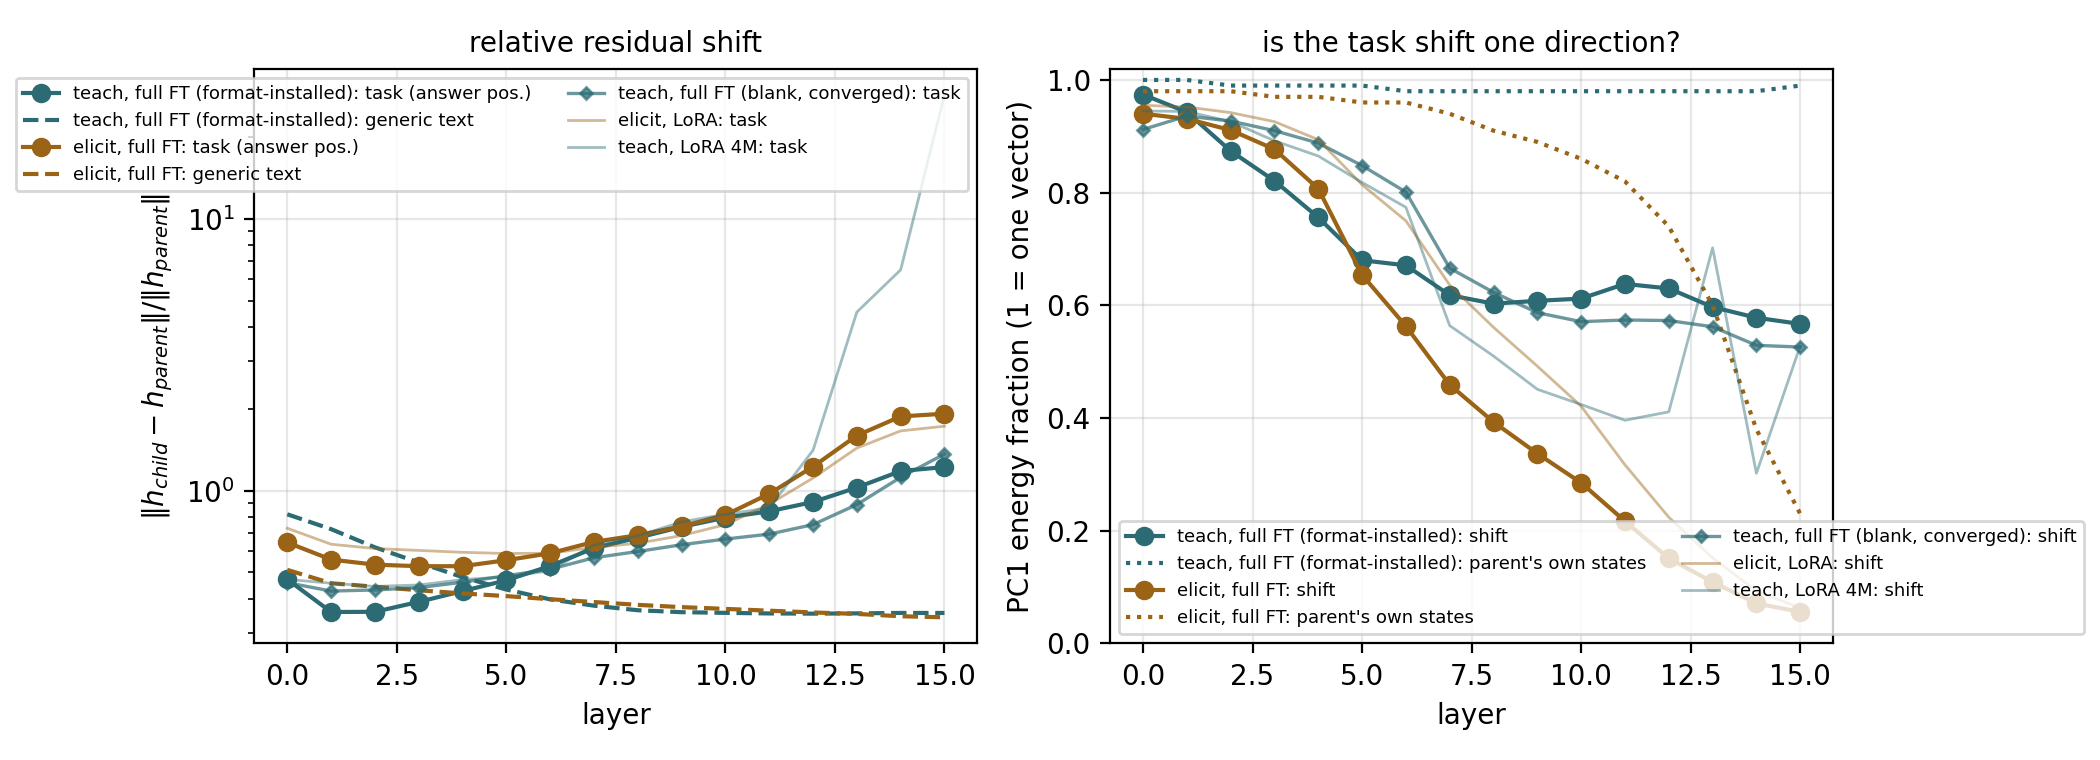
\includegraphics[width=0.95\textwidth]{05_weights/fig_resid_shift.png}
\caption{Full-FT endpoints (thick: elicit vs format-installed teach; diamonds: blank-base teach
converged) with the LoRA endpoints thin. Left: relative residual shift by layer at the answer
position (solid) and on generic story text (dashed). Right: PC1 energy fraction of the 256
per-problem shift vectors, with the parent's own states dotted.}
\label{fig:resid}
\end{figure}
\begin{table}[h]\centering\small
\begin{adjustbox}{max width=\textwidth}
\begin{tabular}{lccccc}
\toprule
 & elicit LoRA 1M & teach LoRA 4M & elicit FT & teach FT, blank (conv.) & teach FT, format-inst. \\
\midrule
final exact match & 0.981 & 0.139 & 0.986 & 0.819 & 0.424 \\
PC1 of shift at the read-out (parent's own states) & \textbf{0.063} (0.23) & \textbf{0.528} (0.98) & \textbf{0.056} (0.23) & \textbf{0.526} (0.98) & \textbf{0.567} (0.99) \\
PC1 after removing answer-token directions & 0.072 & 0.520 & 0.061 & 0.528 & 0.561 \\
cosine of each shift to the mean shift & 0.26 & 0.26 & 0.23 & 0.74 & 0.80 \\
shift at answer position, final layer (relative) & 1.72 & 28.6 & 1.92 & 1.36 & 1.22 \\
KL(parent$\|$child) at the answer position (nats) & 14.3 & 14.0 & 16.4 & 22.0 & 12.3 \\
KL(parent$\|$child) on stories (nats/token) & 0.067 & 0.326 & 0.721 & 1.790 & 1.568 \\
\bottomrule
\end{tabular}
\end{adjustbox}
\caption{Residual-stream shift parent$\to$child at the answer position, 256 problems, fp32.
Blank-base teach FT before continuation: PC1 0.521, final-layer shift 1.42; LoRA-1M teach: PC1
0.351, shift 14.1.}
\label{tab:resid}
\end{table}

% =====================================================================
\end{enumerate}
\section*{D. The latent state: what it means and what it permits before training}
\begin{enumerate}[label=\textbf{M\arabic*}, leftmargin=*, itemsep=1.2em, resume]

\metricsec{Latent reach}{do the words already reach the machinery?}
\what{Whether a natural-language question, before any target training, puts the model's
arithmetic components into the same problem-specific state that the symbols do --- and whether
the model's state is problem-specific at all.}
\how{Render each problem two ways --- \texttt{What is the sum of 621 and 5068?} and
\texttt{621 + 5068 = } --- and record every node's activation at the answer position. Per node:
the mean cosine between the two renderings of the \emph{same} problem minus the mean cosine
between renderings of \emph{different} problems (the ``bridging index''). Positive means the
words put the node into the state the symbols put it in. MLP blocks only: attention heads share
digit tokens across renderings and would score trivially. Compared between the symbol-only
engine (no binding dose) and the elicit parent (binding dose installed). A second, geometry-only
check: how problem-specific the answer-position state itself is, as PC1 and cosine-to-mean across
the 256 problems ($\approx1$ means the same state for every problem).}
\numbers{\textbf{Bridging index.} Symbol-only engine: $\approx0.00$--$0.01$ at every layer.
Elicit parent: $+0.07$--$0.13$ across layers 7--15, about $10\times$. \textbf{State geometry at
the final layer.} Elicit parent: cosine-to-mean $0.51$, PC1 $0.23$ (problem-specific). Blank base:
$0.99$ and $0.98$; format-installed base: $0.99$ and $0.99$ --- the same state for every problem
(emitting a number is not knowing which). \emph{Reading:} before any target training, a
natural-language question already activates the elicit parent's arithmetic MLPs and leaves it in
a problem-specific state; the teach parent has no arithmetic MLPs to activate and is in the same
state for every problem.}

\metricsec{Answer depth}{the answer already there vs.\ absent; finished one layer earlier vs.\ later}
\what{At which layer the answer becomes readable from the model's internal state --- before
training (is it there at all?) and after (how early is it finished?).}
\how{Read the model's intermediate state at each layer as if it were the output, three ways.
\emph{Logit lens}: apply the final unembedding to the layer-$\ell$ state. \emph{J-lens}
(Jacobian lens): first transport the state to the final-layer basis with the average Jacobian
$\partial h_{\mathrm{final}}/\partial h_\ell$ over held-out story text, then unembed --- this
reads what the state is \emph{disposed to make the model say}, and is where the answer can appear
before the model emits it. \emph{R-lens}: the same transport with a relevance-propagation
backward pass, more faithful at early layers. Scored token $=$ the first digit chunk of the
answer (for negative answers the sign is fed in first, so predicting a minus sign never counts).
Per layer: the answer token's median rank among 128K vocabulary entries (chance 64K); the
\emph{logit-diff}, the model's preference for the correct answer over a mismatched problem's
answer, in nats ($0$ $=$ no answer-specific signal); and the \emph{settled depth}, the first
layer from which the token stays top-ranked to the end. Rank without logit-diff can be a number
prior (any number ranks well in a model that emits numbers); the two are read together.}
\numbers{Figure~\ref{fig:lens}, Table~\ref{tab:lens}. \textbf{Before training.} Elicit parent
on the NL task, J-space rank of the answer $2{,}606$ at layer 12, $510$ at layer 14, $174$ in the
actual output, preferring the correct answer by $2.1$ nats --- while it emits a rewrite, not a
number. Blank base: $55$--$80$K at every layer in all three lenses, logit-diff $0.0$.
Format-installed base: rank $452$ at the output because it emits numbers, logit-diff $0.0$ at
every layer --- ``a number is coming'' without ``this number''. \textbf{After training.} The
LoRA-elicited child ranks the answer $139$ / $6$ / $1$ at layers 12 / 13 / 14 and settles at layer
14 --- the parent's own trajectory on symbols ($122$ / $6$ / $1$). Full-FT elicited: $338$ / $8$
/ $1$, settled at layer 14 (quartiles 14--14), top-1 $0.80$ at layer 14. Full-FT taught, blank
base: $4{,}196$ / $1{,}916$ / $79$, settled at layer 15 (quartiles 15--15), top-1 $0.12$ at layer
14 rising to $0.80$ at 15 (converged: $4{,}123$ / $1{,}832$ / $138$, $0.16\to0.84$); from the
format-installed parent: $27{,}044$ / $15{,}058$ / $961$, settled at layer 15, $0.11\to0.54$.
LoRA-taught children: $17$--$20$K at layer 14, then $6$--$8$ at layer 15. \emph{Reading:} the
elicit parent carries the answer in its verbalizable space before any target training and
elicitation only amplifies that read-out; the blank base carries nothing, and a taught model
computes the answer one layer later than the engine even when it solves the task.}
\begin{figure}[h]\centering
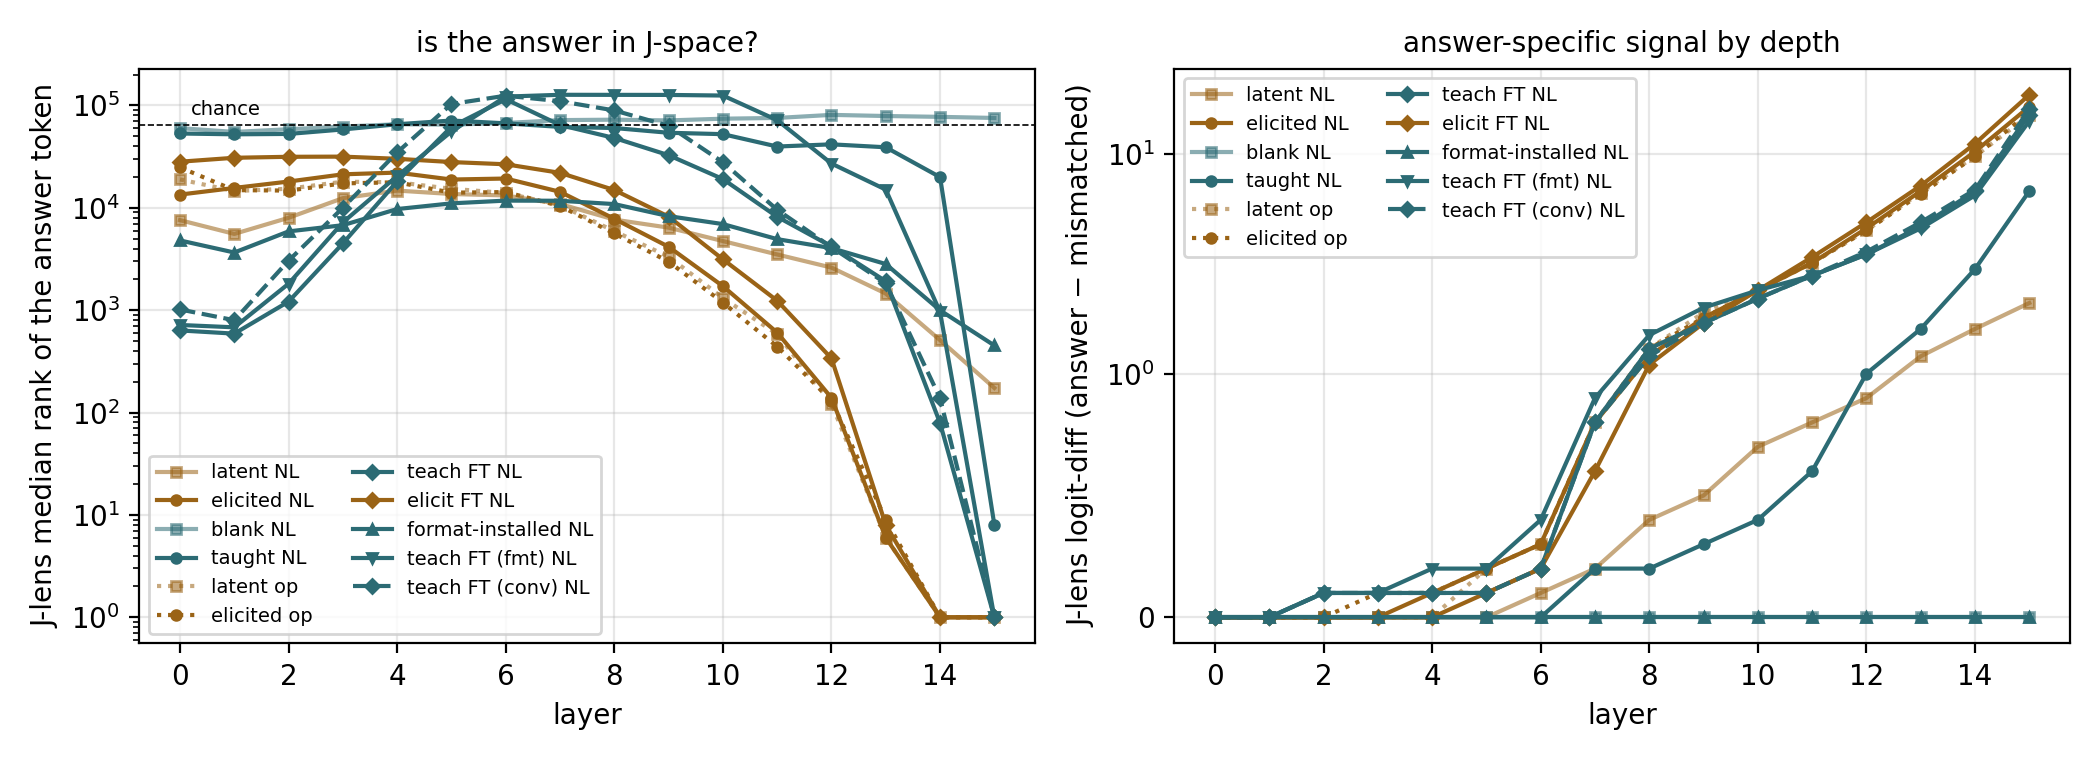
\includegraphics[width=0.95\textwidth]{06_lens/fig_lens_depth.png}
\caption{J-lens read-out of the answer token by layer: median rank (left, chance 64K) and
logit-diff against a mismatched problem's answer (right). Squares = parents, triangles = the
format-installed base and its child, circles = LoRA children, diamonds = full-FT children;
dotted = symbol surface.}
\label{fig:lens}
\end{figure}
\begin{table}[h]\centering\small
\begin{adjustbox}{max width=\textwidth}
\begin{tabular}{llccccc}
\toprule
model & surface & own acc & rank L12 (logit / J / R) & rank L14 (logit / J / R) & read-out & ld \\
\midrule
elicit parent (TS1B-latent) & NL & 0.047 & 5{,}704 / 2{,}606 / 2{,}730 & 436 / 510 / 424 & 174 & $+2.1$ \\
blank base & NL & 0.000 & 76{,}049 / 80{,}840 / 78{,}243 & 77{,}707 / 77{,}320 / 79{,}116 & 75{,}441 & $0.0$ \\
format-installed base & NL & 0.004 & 8{,}394 / 4{,}036 / 5{,}417 & 1{,}106 / 997 / 998 & 452 & $0.0$ \\
elicited child (LoRA) & NL & 0.957 & 1{,}584 / 139 / 464 & 1 / 1 / 1 & 1 & $+16.5$ \\
elicited child (full FT) & NL & 0.988 & 1{,}797 / 338 / 492 & 1 / 1 / 1 & 1 & $+18.7$ \\
taught child (full FT, blank, converged) & NL & 0.844 & 18{,}988 / 4{,}123 / 9{,}620 & 170 / 138 / 459 & 1 & $+16.1$ \\
taught child (full FT, format-installed) & NL & 0.535 & 23{,}909 / 27{,}044 / 25{,}529 & 381 / 961 / 1{,}848 & 1 & $+14.2$ \\
taught child (LoRA 4M) & NL & 0.117 & 54{,}896 / 41{,}722 / 41{,}666 & 40{,}496 / 17{,}183 / 21{,}998 & 6 & $+7.6$ \\
taught child (LoRA 1M) & NL & 0.109 & 51{,}167 / 41{,}677 / 44{,}335 & 35{,}620 / 19{,}933 / 21{,}156 & 8 & $+6.8$ \\
elicit parent (TS1B-latent) & symbols & 0.836 & 1{,}224 / 122 / 334 & 1 / 1 / 1 & 1 & $+15.1$ \\
elicited child (LoRA) & symbols & 0.855 & 1{,}360 / 131 / 399 & 1 / 1 / 1 & 1 & $+15.5$ \\
\bottomrule
\end{tabular}
\end{adjustbox}
\caption{Median rank of the answer's first digit token among 128K entries under the three lenses;
``own acc'' $=$ the model's own first-digit-token accuracy on the 256 problems; read-out $=$ the
last layer, where all lenses equal the model's output; ld $=$ logit-diff at the read-out (nats).
Blank-base teach FT before continuation: 18{,}502 / 4{,}196 / 9{,}429, then 141 / 79 / 377, own
acc 0.797, ld $+15.2$.}
\label{tab:lens}
\end{table}

\metricsec{Switch-on}{can the capability be turned on without training?}
\what{Whether the task can be unlocked in the parent with its weights frozen --- possible only if
the machinery is already there.}
\how{Exact match on the target task under interventions that train nothing. (a) \emph{Self-chain}:
let the parent rewrite the question in its own symbols, then feed it its own rewrite. (b)
\emph{Donor patching}: take the fine-tuned child's activations at the 32 circuit nodes (M2) and
write them into the parent at the answer position, either as one mean vector over problems or as
each problem's own activations (``per-prompt states''); the same with 32 random nodes as control.
``Format'' $=$ the fraction of outputs that are a number at all. Done for the elicit side (child
into the elicit parent) and the teach side (taught child into its own parent: the blank base, or
the format-installed base).}
\numbers{Figure~\ref{fig:ladder}, Table~\ref{tab:steer}. \textbf{Elicit parent}: direct $0.000$;
self-chain $\mathbf{0.328}$ ($=0.484\times0.668$, rewrite accuracy $\times$ symbol accuracy ---
this product held on four model variants); per-prompt states of the LoRA child $0.125$, of the
full-FT child $0.121$ (random nodes: $0.000$); the mean vector changes the output format only.
\textbf{Teach parents}: blank base plus the same doses $0.000$; blank plus chain $0.000$ (a
parser without an engine); taught donor into the blank base $\le0.004$ in every condition, for
all four taught children; the format-installed base with its own taught child's per-prompt
states $0.016$. \emph{Reading:} the elicit parent is one composition step or one activation
patch away from the task because the machinery is there and only has to be switched on; the
teach parents have nothing underneath to switch on, so no patch from any taught model helps.}
\begin{figure}[h]\centering
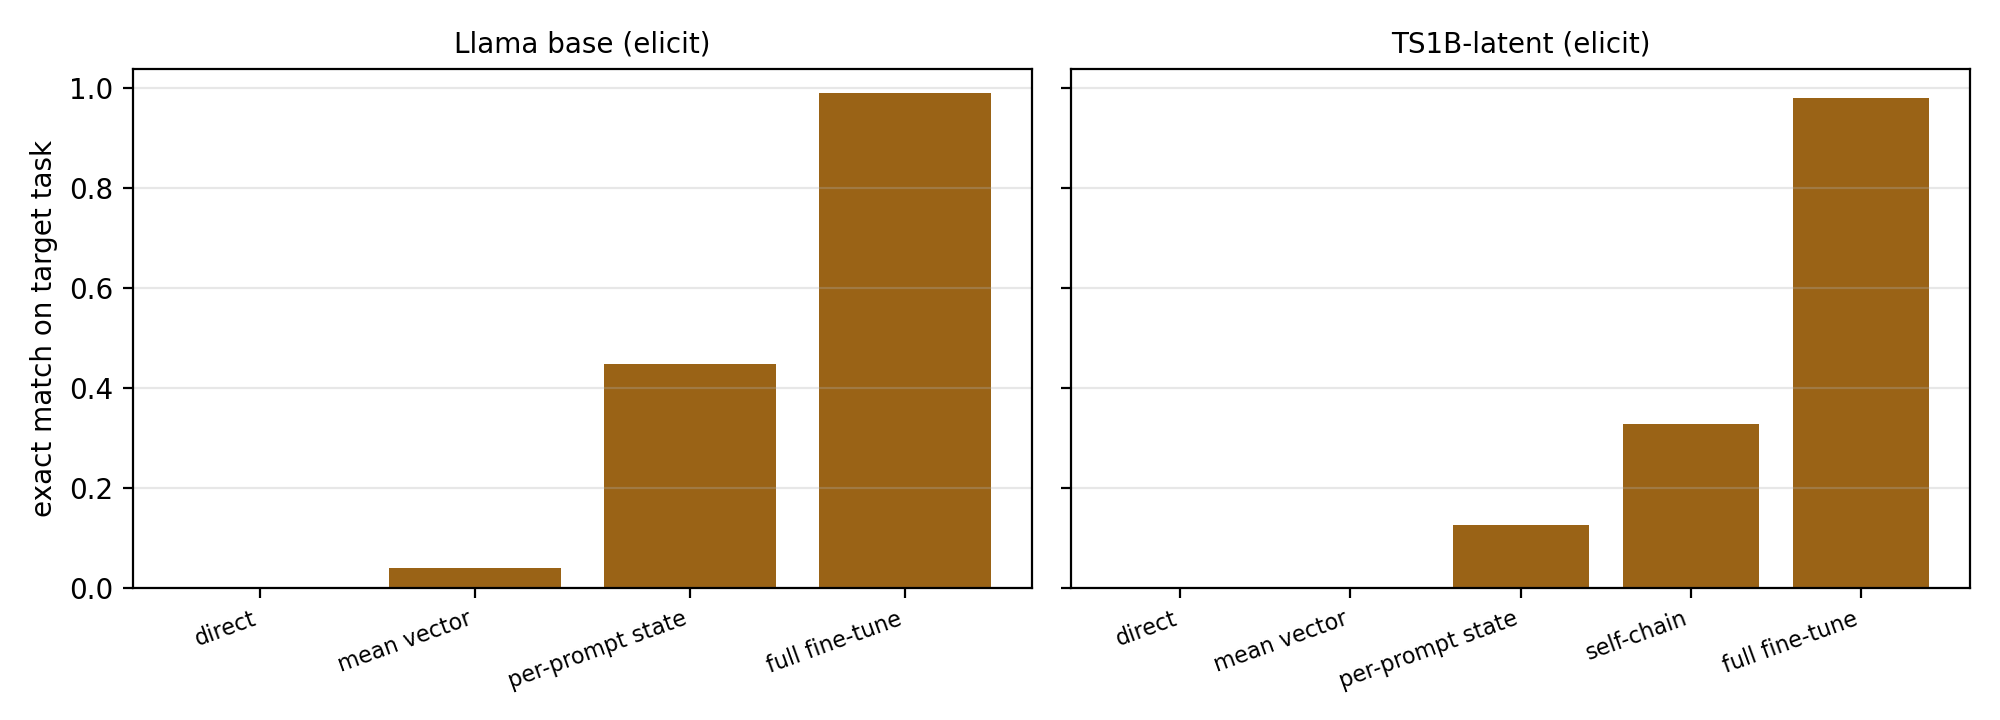
\includegraphics[width=0.55\textwidth]{04_interventions/fig_intervention_ladder.png}
\caption{Intervention ladder on the elicit parent (weights frozen except the last bar).}
\label{fig:ladder}
\end{figure}
\begin{table}[h]\centering\small
\begin{adjustbox}{max width=\textwidth}
\begin{tabular}{llcc}
\toprule
Patient + intervention (32 circuit nodes) & condition & format & exact match \\
\midrule
elicit parent + LoRA child's mean vector & circuit nodes & 0.164 & 0.000 \\
elicit parent + LoRA child's per-prompt states & circuit nodes & 0.359 & \textbf{0.125} \\
 & random-32 nodes & 0.051 & 0.000 \\
elicit parent + full-FT child's per-prompt states & circuit nodes & 0.387 & \textbf{0.121} \\
elicit parent self-chain (no donor) & own rewrite + ``= '' & -- & \textbf{0.328} \\
blank + binding dose, self-chain & parser without engine & -- & 0.000 \\
blank + taught donor (LoRA 1M / LoRA 4M / full FT / converged) & every condition & $\le$0.02 & $\le$0.004 \\
format-installed base + its taught child's per-prompt states & circuit nodes & 0.836 (base 1.000) & 0.016 \\
\bottomrule
\end{tabular}
\end{adjustbox}
\caption{Zero-training interventions.}
\label{tab:steer}
\end{table}

\end{enumerate}

% =====================================================================
\section*{E. Every metric on the full-fine-tune endpoints}

Both regimes under one method. The elicit twin and two teach twins, each fully fine-tuned with
the identical recipe on the identical 4M file to convergence. The format-installed teach twin is
the design-matched comparison (both parents already output numbers); the blank-base teach twin
is the better-performing one. They agree on every row.

\begin{table}[h]\centering\small
\begin{adjustbox}{max width=\textwidth}
\begin{tabular}{lcccl}
\toprule
 & elicit FT & teach FT, format-installed & teach FT, blank (conv.) & metric \\
\midrule
exact match (0-shot) & 0.986 & 0.424 & 0.819 & M1 \\
steps to stop (passes) & 21{,}500 (0.7) & 58{,}500 (1.9) & 72{,}000 (2.3) & M1 \\
held-out test loss (nats/token) & 0.015 & 0.639 & 0.154 & M1 \\
circuit overlap with the elicit-FT circuit & -- & 0.306 & 0.333 & M2 \\
circuit overlap with the LoRA-elicited child & 0.641 & 0.333 & 0.333 & M2 \\
top-8 nodes sufficient / necessary & 0.923 / 0.943 & 0.983 / 0.988 & 0.950 / 0.965 & M3 \\
operand-reading heads vs the parent's engine (first / second) & 0.694 / 0.857 & 0.879 / 0.659 & 0.763 / 0.658 & M4 \\
gradient norm, first 1\% $\to$ last 10\% of steps & 4.80 $\to$ 1.39 (decays 3.4$\times$) & 2.69 $\to$ 3.77 (grows 1.4$\times$) & 2.30 $\to$ 3.43 (grows 1.5$\times$) & M6 \\
cumulative gradient mass & 44{,}021 & 378{,}170 & 353{,}277 (+ 30{,}954) & M6 \\
relative weight write $\|\Delta W\|/\|W\|$ & 0.050 & 0.086 & 0.102 & M7 \\
PC1 of the state shift (after removing answer content) & 0.056 (0.061) & 0.567 (0.561) & 0.526 (0.528) & M8 \\
answer settled depth, median (quartiles) & layer 14 (14--14) & layer 15 (15--15) & layer 15 (15--15) & M10 \\
J-space rank of the answer at layers 12 / 13 / 14 & 338 / 8 / 1 & 27{,}044 / 15{,}058 / 961 & 4{,}123 / 1{,}832 / 138 & M10 \\
child's states patched into its own parent, per-prompt (mean) & 0.121 (format only) & 0.016 (0.000) & 0.004 (0.000) & M11 \\
\bottomrule
\end{tabular}
\end{adjustbox}
\caption{The full-FT endpoints, one row per metric.}
\label{tab:ftpair}
\end{table}

\section*{Notes on measurement}

\begin{itemize}[nosep]
  \item \textbf{Teach-side metrics were re-measured on performing taught models.} The first
    taught endpoint (LoRA 1M, exact match 0.093) had not learned the task. Every teach-side
    metric was re-run on the LoRA-4M and the three full-FT taught endpoints, with the full-FT
    elicited endpoint as the method control. Three earlier readings changed and are stated in
    their revised form above: taught operand roles are mostly shared rather than absent (M4), the
    circuit difference is partial rather than total (M2), and the size of the taught state shift
    depends on the fine-tuning method (M8).
  \item \textbf{Answer depth is scored on the first digit token.} Scoring the raw first token
    credited a taught child with layer-5 formation on 48 problems --- all subtractions with a
    negative answer, whose first token is the minus sign, produced by a comparison circuit. With
    the sign fed in first the effect vanishes; the other models were unaffected.
  \item \textbf{Construction controls.} The same doses on the blank twin change nothing on the
    target (0.000 in every probe); a sum-only binding dose leaves ``difference'' unbound; the
    composition law self-chain $=$ rewrite $\times$ compute held on four variants.
\end{itemize}

\end{document}
